\chapter{Reservoir Networks}\label{ch_reservoir}
\chapterauthor{Zo\"e Tosi, Jeff Yoshimi}{.9,.1}

% Need a proper intro, and then subsections

% Integrate the material from drive: https://docs.google.com/document/d/1dZJUnC6AnCKxJlid4h_b3MN11bgb3rGlyUjNneK7TVs/edit

% Pass needed on this section getting everything a consistent length
% Mention spiking Liquid State Machines vs. ESN. Also ESN more machine learning and LSM more comp. bio (so connect to older distinctions)
% Reservoir like a hidden layer
% Use quote from Mondares: ``"The word liquid in the name comes from the analogy drawn to dropping a stone into a still body of water or other liquid. The falling stone will generate ripples in the liquid. The input (motion of the falling stone) has been converted into a spatio-temporal pattern of liquid displacement (ripples)." (Links to an external site.)Links to an external site.''

% Discuss spectral radius? Easy to use in Simbrain 4.  Good to be slightly less than 1. http://danielrapp.github.io/rnn-spectral-radius/

% The reservoir itself is not often trained, but it can be. A cool example, the allostatic update rule (Falandays et. al). Include pictures

Another approach to training recurrent networks is to, in essence, \emph{not train them at all}, using a technique known as \glossary{reservoir computing}. RNNs offer a suite of advantages over their feed-forward cousins owing to their potential ability to store information about past stimuli which is made possible by recurrent connectivity. Because feedback connections exist, the current state of the nodes in the recurrent portion of the network (and any information it contains about prior inputs or states) becomes part of the input in determining the next state of those nodes. They become ideal, then, for processing time-series data (as opposed to simple pattern association tasks). 

%  Being high-dimensional dynamical systems means that they can express a wide variety of dynamical regimes which may or may not be helpful with respect to the task at hand. 
% Add discussion of vanishing gradients
However, the kind of internal dynamics which make RNNs desireable (they have a ``life of their own'') also makes them difficult to effectively use. Throughout the 1980s and 1990s the problem of how to properly train RNNs prevented them from being used on a wider scale. How exactly the recurrent weights should be altered in response to an error signal was largely unclear. In 2001 two separate researchers, Herbert Jager and Wolfgang Maass, a computer scientist and neuroscientist respectively, independently came to the conclusion that the reverberating internal dynamics within the recurrent portion of a network could be harnessed \emph{without training the recurrent weights} so long as certain constraints were imposed on the networks in question. That is, instead of formally training the recurrent weights and trying to calculate what node activations should be in a likely chaotic system, why not bypass the issue entirely by instead simply focusing on putting the recurrent portion into a \emph{helpful dynamical regime}. But what would such a regime look like? Does such a thing even exist? If so, how does one go about imbuing a RNN with it?

The answers to these questions can be found in a humble pond of water. Suppose you're standing in front of a pond on a cool autumn day. There is no wind, the multitude of  water-dwelling insects of summer have gone into hiding for the winter, and the fish have no reason to breach the surface. It is in fact so placid that the pond could be mistaken for an oddly shaped mirror reflecting the sky above. You notice a few pebbles by your feet and, perhaps uncomfortable with just how still this scene is before you, you decide to pick one up and toss it into the water. It makes a small splash and ripples emanate in a ring from where the pebble plopped down. The ripples eventually reach the edge of the pond and are reflected back toward the center, the tiny waves interfere with one another creating a striking pattern given the former stillness of the pond. But as they continue to reverberate across the pond's surface they become smaller, less defined, and eventually the pond returns to its placid state--as if you'd never thrown the pebble at all. 

You decide to toss in another pebble, but this time you throw a little harder. As before, the pebble plops into the pond, but this time significantly further away. Once again, ripples emanate from the place where the pebble dropped, but this time--being as it is, closer to the other side of the pond--some of the ripples reach the water's edge opposite you sooner, reflect back, and after a few moments you realize the patterns of ripples on the surface this time are \emph{completely different} than before. You throw another stone... this time it lands mere centimeters from where the original pebble did. The ripples radiate outward once more and as far as you can tell are nearly indistinguishable from those that came from the first pebble you threw. The ripples reflect back, slightly differently from the first time, but to your surprise after mere moments the pattern of ripples on the water's surface is different from the ones produced by either of the two previous stones, though much closer to the pattern produced by the first stone. This is because when you drop a stone into the pond the perturbation to the water's surface is \emph{unique} to the location where the stone was dropped. Proximal drop locations produce similar patterns of ripples that remain more similar for longer amounts of time, while spatial distant ones are immediately completely different. Note the following: You did not have to do anything to this pond for this to be the case; it is simply \emph{an intrinsic property} of fluids. It arises from the fact that the pond is 1) responsive to external perturbation, 2) all perturbations eventually die out, with the pond returning to its initial unperturbed state, and 3) that the dynamics of the system (water molecules and surface tension) respond consistently to the same perturbation yet are complex enough that different perturbations produce different states. This doesn't just apply to where a single stone has been dropped into the pond, for if one stone was thrown right after another the pattern of ripples would be unique to \emph{where and when} the two stones were thrown relative to one another, with the effects of the more recently dropped stone taking longer to dissipate than those of its earlier counterpart. This means that the pattern of ripples on the surface of our pond at any given time actually represents (i.e. contains information concerning) the \emph{history} of perturbations to the pond! An example of this representational capacity was concretely demonstrated in \cite{fernando2003pattern} where a literal bucket of water was used for nonlinear pattern separation \ref{F:bucketclassifier}.

Suppose you come back to the pond in the dead of winter. Now when you toss a stone at the pond they create tiny ablations on the hard surface, but unlike when the surface was liquid, the points of impact do not change over time. There is no way to tell how long ago you dropped the stones or in what order because the system doesn't respond meaningfully to external perturbations beyond the initial point of impact. Any pattern of marks on its surface could've arisen at any point in time after it froze and in any order. The ice simply sits there, solid, unchanging, and impregnable. The surface of the pond has lost its spatiotemporal representational capacity by being frozen--perfect for ice skating--though perhaps less interesting in and of itself. Dynamically this is referred to as an \emph{ordered} regime.

% Consider making regime types glossary items

% Earlier longer text: Later you decide to come back to the pond in the dead of winter. It's a frigid day, but determined to get out of the house and exercise you decide to venture to the pond in the hopes that it will be frozen over enough for some ice skating. The icy wind lacerates your cheeks, but you make it there. To your disappointment, however, you can't quite tell if the pond is frozen through enough for skating. Thinking back to your autumn foray with the pebbles you realize that you can test the stability of the ice with the aid of some, perhaps larger, pebbles. After a moment of searching you happen upon two large rocks. Gathering your strength and heaving with both arms you throw the first which lands in the center of the pond with a loud thud. The ice holds with no visible cracks emanating from where the rock had been hurled. Just to be extra sure you throw the second one, which like the first lands with a loud thud, and likewise fails to break the surface or cause noticeable cracking. Satisfied that it is safe to ice-skate on the pond you walk triumphantly over to the two stones to remove them from the ice lest you trip over them later. Beneath each, however the surface of the ice has been damaged... little scars on the surface remain where each stone ablated some ice upon their respective impacts. The surface of the ice reflects where the stones were dropped, yes, but unlike when the surface was liquid, the points of impact do not change over time. There is no way to tell how long ago you dropped the stones or in what order because the system doesn't respond meaningfully to external perturbations beyond the initial point of impact. Any pattern of marks on its surface could've arisen at any point in time after it froze and in any order. The ice simply sits there, solid, unchanging, and impregnable. The surface of the pond has lost its spatiotemporal representational capacity by being frozen--perfect for ice skating--though perhaps less interesting in and of itself. Dynamically this is referred to as an \emph{ordered} regime, which will be important later.

\begin{figure}[h]
\centering
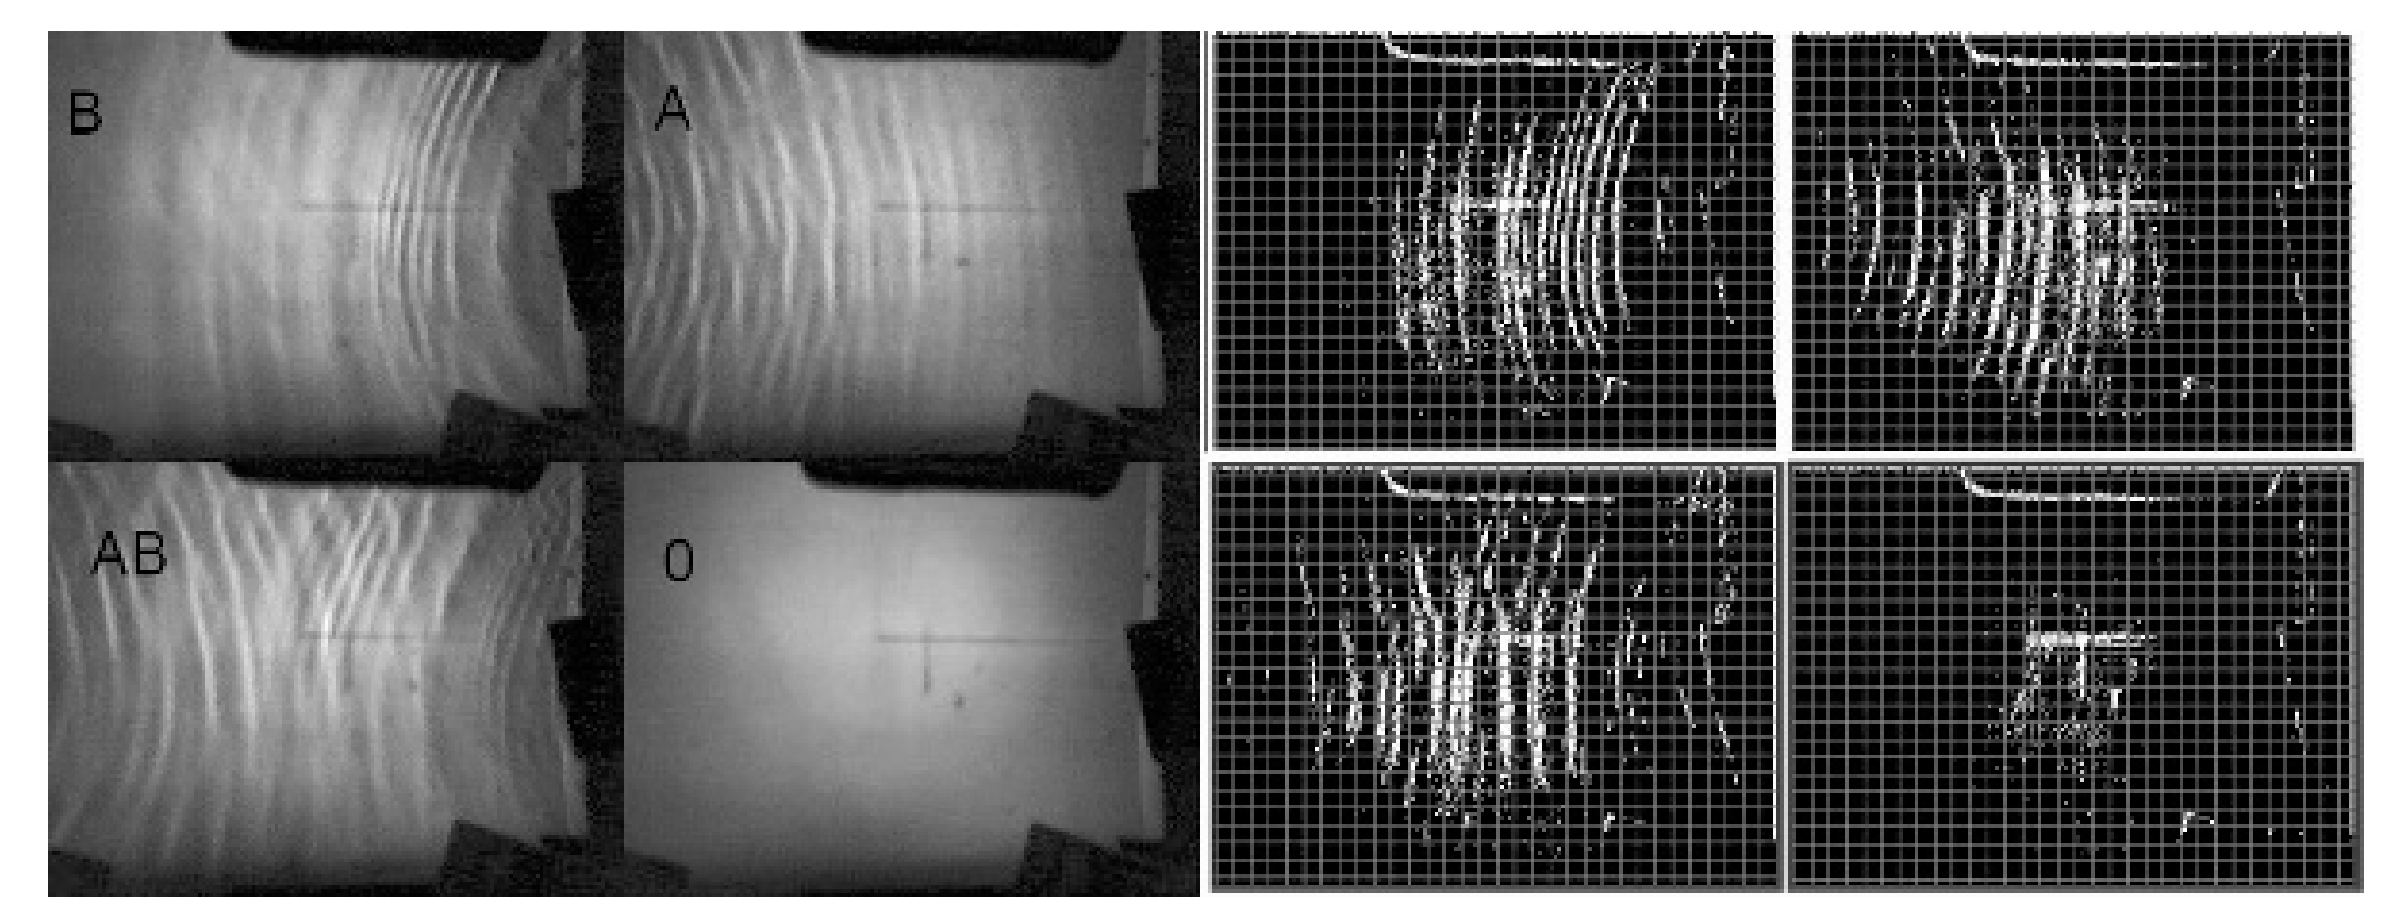
\includegraphics[width=0.6\textwidth]{images/BucketPatternRecognition.png}
\caption[Fernando, Chrisantha and Sojakka, Sampsa.]{Pattern recognition has literally been done in a bucket of water, providing a concrete example of the water metaphor. Ripples on the surface were recorded in response to labelled inputs (perterbations emanating from the left or right side of the bucket, and when combined with a perceptron classifier was able  to perform nonlinear pattern separation (XOR). Retrieved from \cite{fernando2003pattern}. }
\label{F:bucketclassifier}
\end{figure}

After your afternoon of ice-skating, you once again brave the harsh, icy winds, and return home. Hungry, cold, and tired, nothing sounds better than a nice bowl of soup. You head to the kitchen, grab a pot, fill it with water, and then place it atop the stove. Setting the burner to high you stand in front of the pot, warming yourself while waiting patiently for the water to boil. Initially it's as still as the autumn pond. You tap the water's surface with a wooden spoon and watch as the ripples emanate from the point of contact, peacefully expanding out, hitting the walls, reflecting, interfering, and eventually dying out exactly as you remember. As time goes by, little bubbles form on the bottom of the pot, turning to larger bubbles, and before you know it the water in the pot has been brought to a rolling boil. Its surface constantly bubbles, always moving--a stark contrast to its prior stillness. You look at the complex and ever changing structure on the surface of the boiling water, and realize just how unlikely it is that at any previous time the water looked \emph{exactly} as it does now. You forcefully, but carefully drop in the bottom of your spoon. You can see small waves from the point of contact, but only for a brief instant as they are fully consumed and incorporated into the surrounding disorder. Curious, you aim your spoon well and make contact with the surface just as forcefully before and as close as you could to the last place where you dropped the spoon. To no one's surprise once again small waves are created which quickly dissipate into the chaos of the churning, bubbling, liquid in the pot. Consistent with your realization from before, it is apparent that despite dropping in your spoon with the exact same amount of force and in the exact same position, the state of the surface of the water before you has likely never looked exactly like this before and is \emph{completely different} from its state in the same interval of time after your first spoon drop. The water, in its excited state, has taken on a life of its own--one which incorporates your perturbations, but which is unpredictable--assigning completely unique states to even the same perturbation. The water has lost it's spatiotemporal representational capacity by boiling. Dynamically this is referred to as the \emph{chaotic} regime, and just as with the \emph{ordered} regime it is largely useless from the perspective of reliably representing past inputs.

If the boiling pot was in a chaotic regime and the frozen pond was in an ordered regime, then how would we describe the liquid surface of the pond all those months ago? The answer is: the \emph{edge of chaos}, a dynamical regime where the system is affected by perturbations, but the differences between the states produced by the perturbations and the perturbations themselves remain largely constant. Figure \ref{F:edgechaos} gives us an example of the sorts of activity we expect to find as well as the conditions necessary to produce their respective dynamical regimes in an actual neural network as opposed to liquid (or solid) water. 

\begin{figure}[h]
\centering
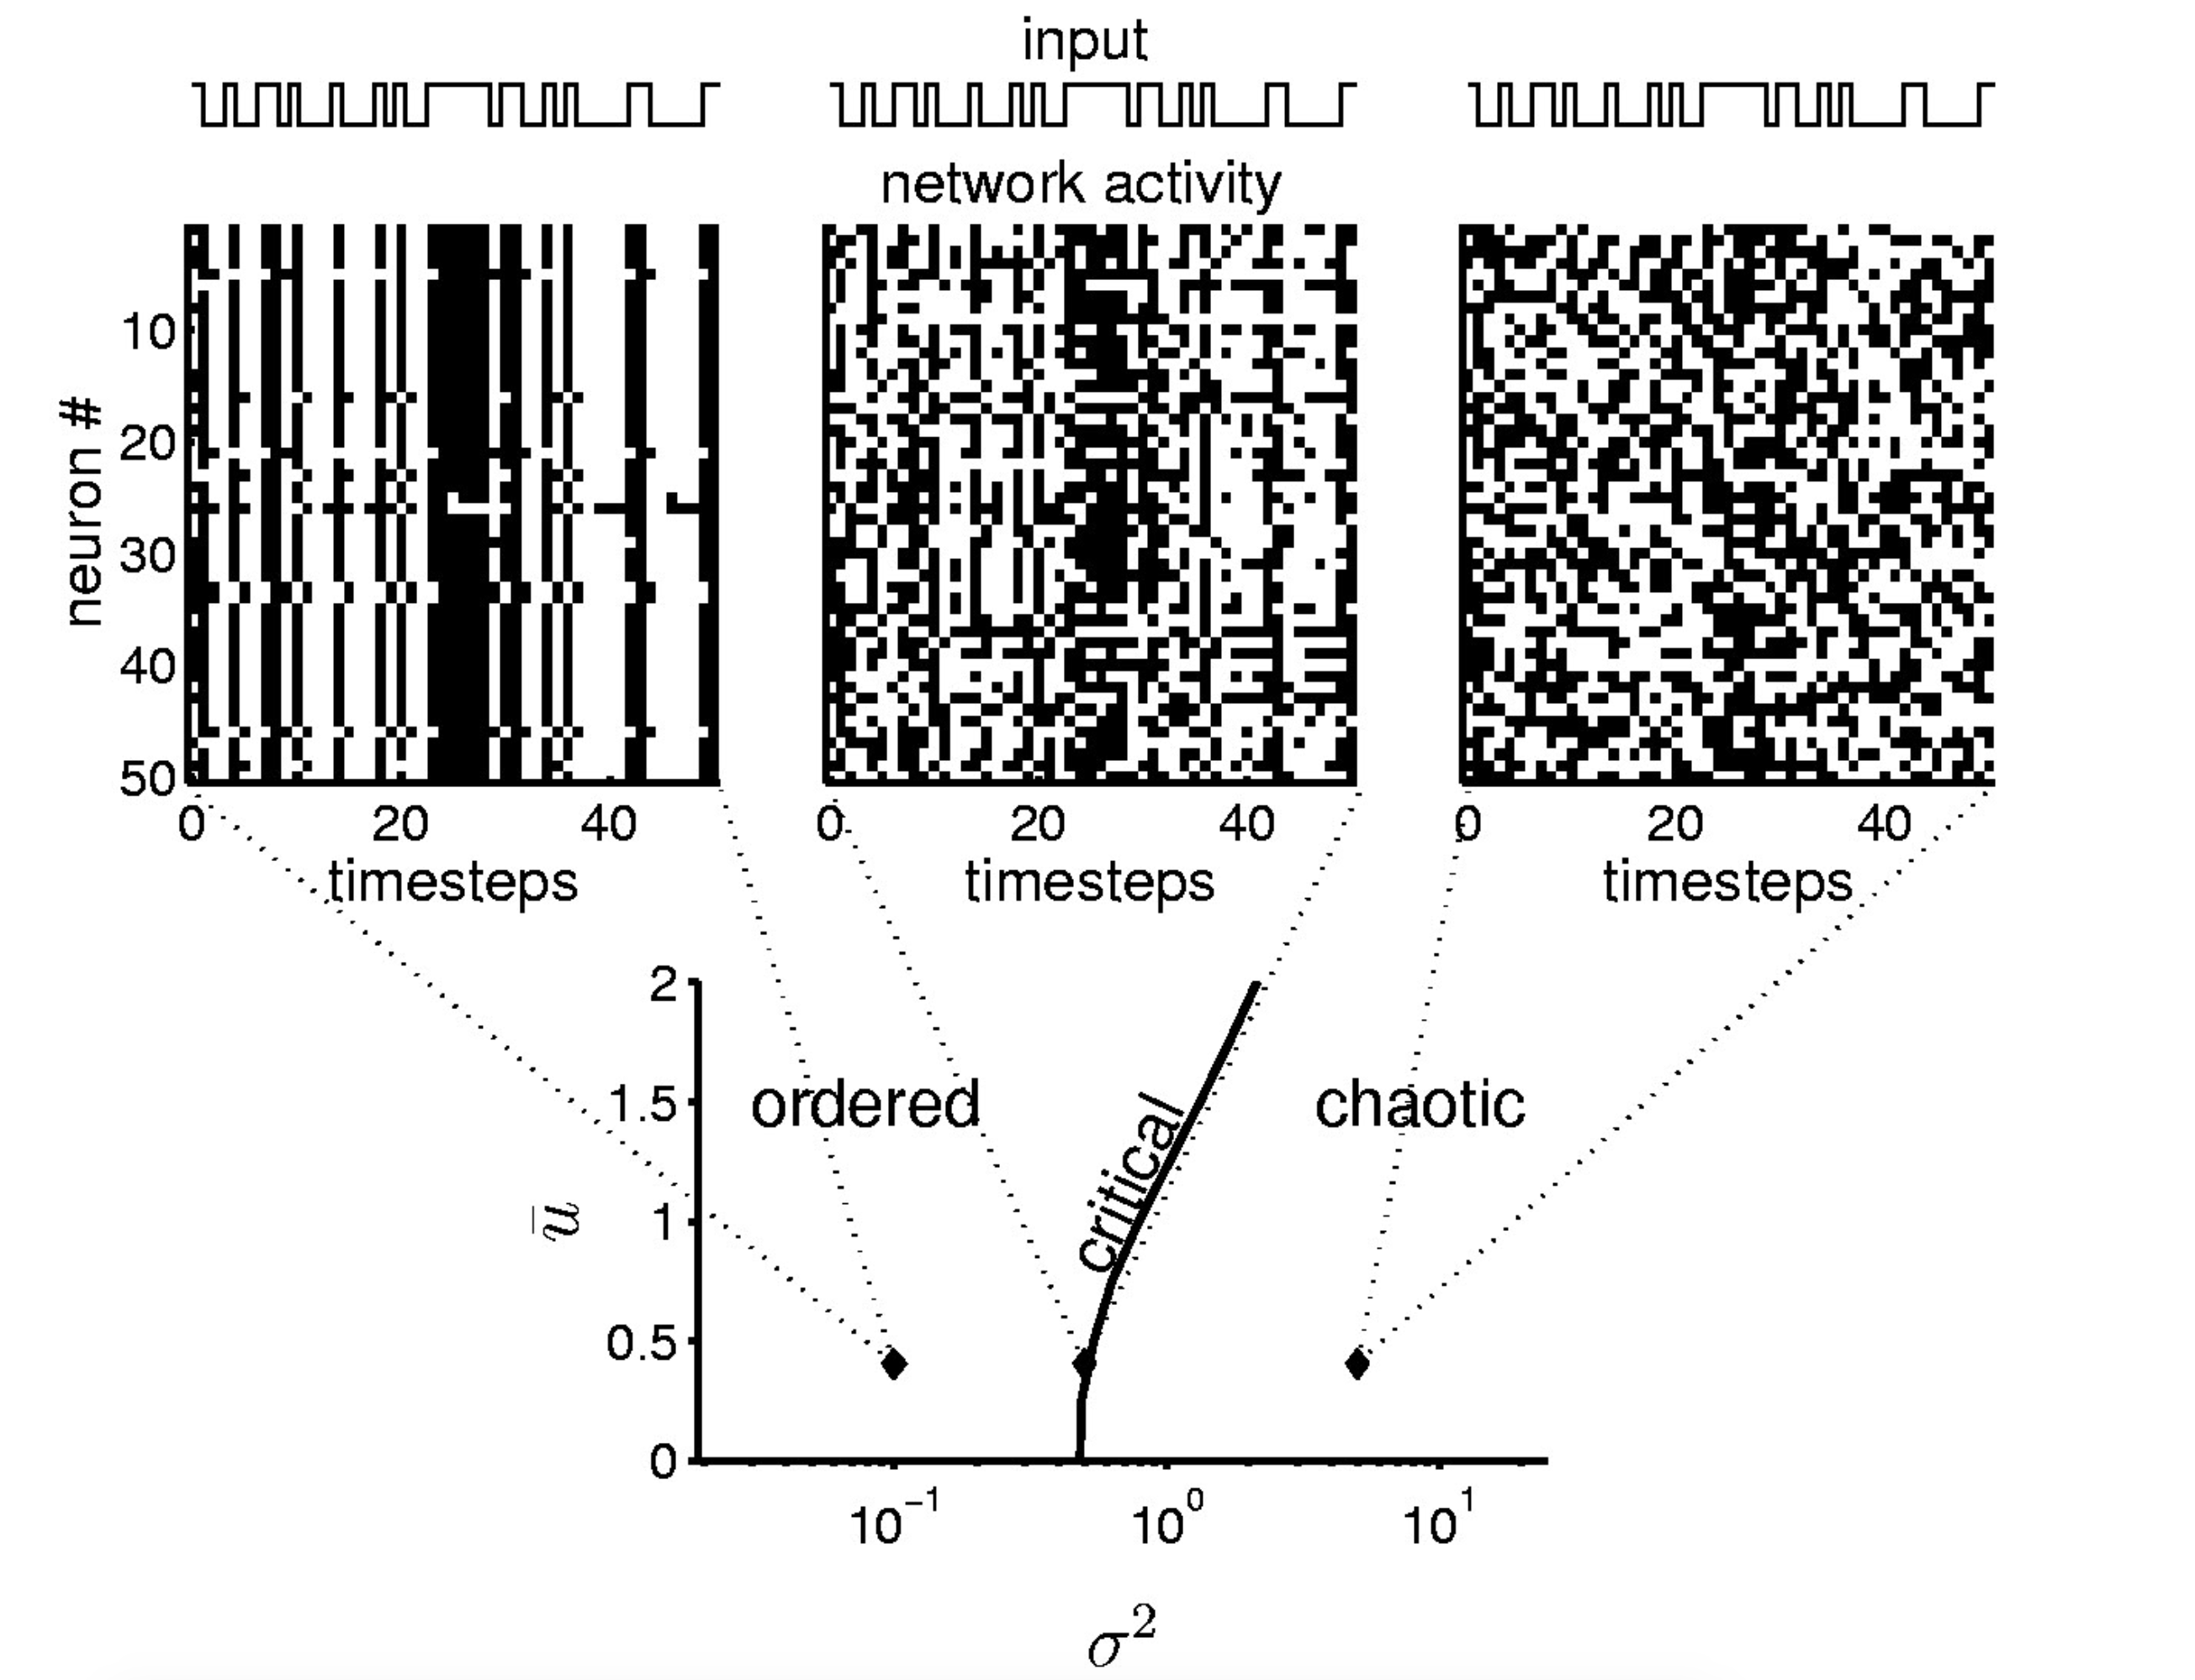
\includegraphics[width=0.6\textwidth]{images/EdgeOfChaos.png}
\caption[Nils Bertschinger and Thomas Natchl\"ager]{Here we have an example of ordered, chaotic and edge-of-chaos dynamical regimes in a recurrent neural network as well as what portions of the network's parameter space in terms of the variance of weights ($\sigma^2$) and the mean value of the input signal ($\bar{\mu}$) Notice the similarities in the network's responses to an input signal (top row) and the pond metaphor used previously. The left-hand side gives us a network that presents no or very little information on time-series and is only capable of representing the current input. For the toy network used in \cite{bertschinger2004real} the ordered regime occurs when the variance of the weights is low and/or the input signal is strong. The right-hand side gives us a network whose activity is dominated by its own internal dynamics, which is not consistently or obviously responsive to the input time-series. Likewise this dynamical regime is produced by high variance among the recurrent weights and typically weaker input signals.The middle plot represents the ideal dynamical regime for these networks because it responds to the input signal, but also has some autonomous internal dynamics which are capable of preserving information about previous entries in the time-series. Networks with this property occupy a specific manifold in the parameter space of variance on the weights and strength of the input signal. Image retrieved from \cite{bertschinger2004real}.}
\label{F:edgechaos}
\end{figure}

This representational capacity comes ``for free'' as it were, given the nature of the material in question. What if we could imbue recurrent neural networks with those same properties, i.e. the intrinsic ability to represent perturbations as transients? Instead of peaks and troughs across the surface of water, could not the same sort of thing be accomplished with activity across a recurrent network? What sorts of constraints would need to be placed on the network for such a thing to be possible? What properties must it possess and how can we describe those properties? These are the questions that Wolfgang Maass and Herbert Jaeger independently asked themselves. Instead of training recurrent weights to reduce error, the problem then was how to ``tune'' the network such that it would possess these properties, thus requiring no explicit training, beyond a linear classifier which would simply learn to distinguish different patterns of activity in the so-called dynamical reservoir. In fact Wolfgang Maass found that recurrent spiking neural networks held to some minimal biological constraints actually possessed this property intrinsically, while Herbert Jager was able to derive a set of theorems for constraints on the recurrent weight matrix in a connectionist-style network which guaranteed a fading memory and therefore this property (called "the echo-state property" by Jaeger). 

 There are two main kinds of reservoir networks: echo state networks and liquid state machines (the basic difference is that liquid state machines use spiking neurons). A picture of an echo state network is shown in Fig. \ref{F:esn}. The idea is to take a recurrent network (the ``reservoir'') and see what we can get it to do by driving it with inputs. Reservoir computers are somewhat neurally realistic: the central reservoir is a recurrent network, like the kind of networks found in the brain, and the brain's recurrent networks are typically driven by inputs from other world or from the external world.

\begin{figure}[h]
\centering
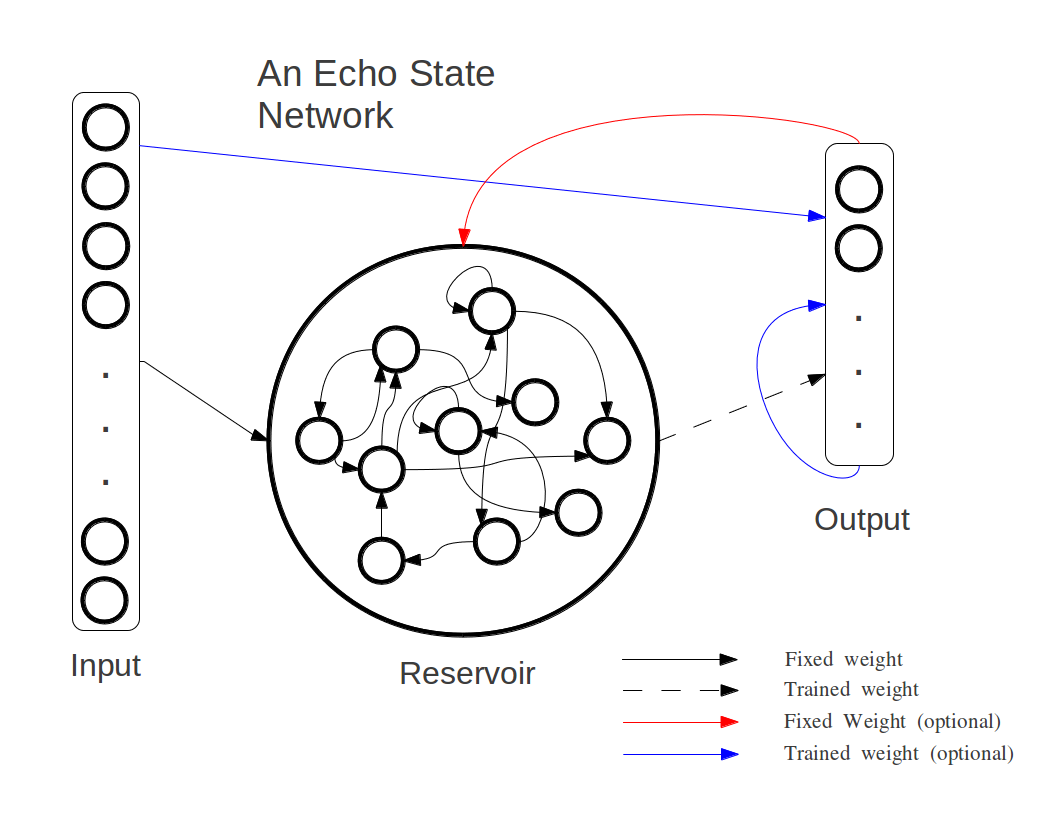
\includegraphics[width=0.6\textwidth]{images/ESNDiagram.png}
\caption[Zo\"e Tosi.]{An echo state network, which is one kind of reservoir computing network.}
\label{F:esn}
\end{figure}

% Creating high-dimensional projections of low dimensional temporally extended inputs such that (ideally) those inputs become linearly separated. // Designed to operate in an ever changing environment and naturally accept temporal streams as input. They can respond to stimuli in real-time in a very natural way. 

The input nodes of an echo state network or liquid state machine drive a reservoir, which is an arbitrary recurrent network, like one of the networks discussed in chapter \extref{ch_dst}. Recall that those networks produce all kinds of interesting dynamical patterns, \eg $n$-cycles of various lengths (2-cycles, 10-cycles, 100-cycles) and even chaotic behaviors. Recall that unfolding patterns in a recurrent network correspond to trajectories in an activation space. Here we have trajectories in the activation space of the reservoir. The inputs change which trajectory the system is following.\footnote{ The reservoir's activity at any moment can be thought of as a high dimensional spatial representation of a lower dimensional time-series over some interval which constitutes its effective memory capacity. Recall that we focused before on dimensionality \emph{reduction}. Here we are going from lower to higher dimensions, which can be useful for classifying temporally extended input streams. States that are not linearly separable in a lower dimensional space can often be separated by a hyperplane through a higher dimensional one. That is the dynamical reservoir can be thought of as taking nonlinearly separable lower-dimensional time-series and projecting them into a higher dimension where they are linearly separable. Hence the only training that is required is the rather efficient training of output weights.}  The trajectories induced by the input stream produce states that can then be classified using the output layer, a ``readout'', which is trained using LMS or a related algorithm. 

Again we are just reusing existing ideas, combining a recurrent network with a few feed-forward networks and training some of the weights using the least mean squares algorithm. We are basically training a network to associate reservoir states with desired readout states, and thereby to associate trajectories in the reservoir activation space with trajectories in the output space.\footnote{Our training dataset $D=(I,T)$ has the same form as usual, but behind the scenes we can use it to create a second training dataset, $D'=(I',T')$, where $T=T'$, and where the $i$th input vectors in $I'$ corresponds to the states produced in the reservoir when it is exposed to the corresponding $i$th input vector in $I$.}  Reservoir networks can be used to classify temporally extended inputs (\eg say what kind of music is being played) or to generate a particular type of input (\eg the input is a frequency and the output is a sine wave at that frequency). 
% Helpful comment here: https://www.researchgate.net/post/what_is_the_realitionship_between_deep_learning_methods_and_reservoir_computing_if_any

A primary goal of reservoir computing is to understand the computational power of the kinds of recurrent networks we see in brains. This is useful for the scientific project of understanding what the theoretical properties of brain networks are. It's also a research project in machine learning. It may be that reservoir computers end up having advantages over other trained recurrent networks, \eg supervised recurrent networks, which we discuss next (which can be very computationally demanding). This is because they use very simple components. The output is just a linear classifier (trained using a variant of LMS) which is faster to use than supervised recurrent methods.\footnote{The problem, however, is that it's not clear how one goes about making a good reservoir, which is an active research topic}.
	